%% begin: LaTeX-Einfeuhrung.tex
\chapter{Einleitung}
\label{chap:Einleitung}
\section{Dokumentaufbau}
\label{sec:Einleitung:Dokumentaufbau}
\lipsum[1-2]
\section{Die Geschichte von \texttt{KOMA-Script}}
\label{sec:Einleitung:Geschichte}
\lipsum[1-2]
\section{Installation}
\label{sec:Einleitung:Installation}
\lipsum[1-2]
\section{Fehlermeldungen, Fragen, Probleme}
\label{sec:Einleitung:Fehlermeldung, Frage, Probleme}
In Kap. \ref{chap:Einleitung} wird \ldots{}.\par%
Das ist ein Test.\par\smallskip
Das war ein \verb|\parsmallskip|.
\lipsum[1-2]
\lipsum[1-3]
\lipsum[1-4]


\part[Einführung in \LaTeX{}, KOMA-Script für Autoren\texorpdfstring{, \cite{LabenbacherTeX}}{}]{Einführung in \LaTeX{}, KOMA-Script für Autoren\texorpdfstring{, \cite{LabenbacherTeX}, \protect\footnote{In \texttt{part}.}}{}}%
\label{part:Einfuehrung in LaTeX, KOMA-Script fuer Autoren, scrbook}%
\chapter[Satzspiegelberechnung mit \texorpdfstring{\TUMstyle{package}{typearea.sty}}{typearea.sty}]{Satzspiegelberechnung mit \TUMstyle{package}{typearea.sty}\texorpdfstring{, \protect\footnotemark{}}{}}\footnotetext{In \texttt{chapter}.}%
\label{chap:Einfuehrung:Satzspiegelberechnung}%
% mbox, only due to underlineing :P
\section[Grundlagen der Satzspiegelkonstruktion]{Grundlagen der Satzspiegelkonstruktion\texorpdfstring{, \cite{LabenbacherTeX}, \ref{sec:Einfuehrung:Hauptklassen:Abgrenzung}, \eqref{equ:Mathematik:E = mc2}}{}\texorpdfstring{, \protect\mbox{\footnotemark}}{}}\footnotetext{In \texttt{section}.}%
\label{sec:Einfuehrung:Satzspiegelberechnung:Grundlagen}%
\subsection[Weiterentwicklung]{Weiterentwicklung\texorpdfstring{, \protect\mbox{\footnotemark}}{}}\footnotetext{In \texttt{subsection}.}%
\label{subsec:Einfuehrung:Satzspiegelberechnung:Grundlagen:Weiterentwicklung}%
\subsubsection[Endstation\texorpdfstring{ (nicht erlaubt in Büchern eigentlich ab incl. hier!)}{}]{Endstation\texorpdfstring{ (nicht erlaubt in Büchern eigentlich ab incl. hier!)}{}\texorpdfstring{, \protect\footnotemark}{}}\footnotetext{In \texttt{subsubsection}.}%
\label{subsubsec:Einfuehrung:Satzspiegelberechnung:Grundlagen:Weiterentwicklung:Endstation}%
\paragraph[Abschnitt]{Abschnitt\texorpdfstring{, \protect\footnote{In \texttt{paragraph}.}}{}}%
\label{para:Einfuehrung:Satzspiegelberechnung:Grundlagen:Weiterentwicklung:Endstation:Abschnitt}%
\minisec{Miniüberschrift ohne Referenzierung}
\lipsum[1-1]%
\section{Satzspiegelkonstruktion durch Teilung}%
\label{sec:Einfuehrung:Satzspiegelberechnung:Satzspiegelkonstruktion Teilung}%
\lipsum[1-1]
\section{Satzspiegelkonstruktion durch Kreisschlagen}
\label{sec:Einfuehrung:Satzspiegelberechnung:Satzspiegelkonstruktion Kreisschlagen}
\lipsum[1-1]
\section{Frühe oder späte Optionenwahl}
\label{sec:Einfuehrung:Satzspiegelberechnung:Optionenwahl}
\lipsum[1-1]
\section{Kompatibilität zu früheren Versionen von \texttt{KOMA-Script}}
\label{sec:Einfuehrung:Satzspiegelberechnung:Kompatibilitaet}
\lipsum[1-1]
\section{Einstellung des Satzspiegels und der Seitenaufteilung}
\label{sec:Einfuehrung:Satzspiegelberechnung:Einstellung Satzspiegel}
\lipsum[1-1]
\section{Einstellung des Papierformats}
\label{sec:Einfuehrung:Satzspiegelberechnung:Einstellung Papierformat}
\lipsum[1-1]
\section{Tipps}
\label{sec:Einfuehrung:Satzspiegelberechnung:Tipps}
\lipsum[1-1]

\chapter{Die Hauptklassen \texorpdfstring{\TUMstyle{package}{scrbook, scrreprt, scrartcl}}{scrbook, scrreprt, scrartcl}}
\label{chap:Einfuehrung:Hauptklassen}
\section{Frühe oder späte Optionenwahl}
\label{sec:Einfuehrung:Hauptklassen:Optionenwahl}
\lipsum[1-1]
\section{Kompatibilität zu früheren Versionen von \texttt{KOMA-Script}}
\label{sec:Einfuehrung:Hauptklassen:Kompatibilitaet}
\lipsum[1-1]
\section{Entwurfsmodus}
\label{sec:Einfuehrung:Hauptklassen:Entwurfsmodus}
\lipsum[1-1]
\section{Seitenaufteilung}
\label{sec:Einfuehrung:Hauptklassen:Seitenaufteilung}
\lipsum[1-1]
\section{Wahl der Schriftgröße für das Dokument}
\label{sec:Einfuehrung:Hauptklassen:Wahl Schriftgroesse}
\lipsum[1-1]
\section{Textauszeichnungen}
\label{sec:Einfuehrung:Hauptklassen:Textauszeichnungen}
\lipsum[1-1]
\section{Dokumenttitel}
\label{sec:Einfuehrung:Hauptklassen:Dokumenttitel}
\lipsum[1-1]
\section{Zusammenfassung}
\label{sec:Einfuehrung:Hauptklassen:Zusammenfassung}
\lipsum[1-1]
\section{Inhaltsverzeichnis}
\label{sec:Einfuehrung:Hauptklassen:Inhaltsverzeichnis}
\lipsum[1-1]
\section{Absatzauszeichnung}
\label{sec:Einfuehrung:Hauptklassen:Absatzauszeichnung}
\lipsum[1-1]
\section{Erkennung von rechten und linken Seiten}
\label{sec:Einfuehrung:Hauptklassen:Erkennung rechts links}
\lipsum[1-1]
\section{Kopf und Fuß bei vordefinierten Seitenstilen}
\label{sec:Einfuehrung:Hauptklassen:Kopf und Fuss}
\lipsum[1-1]
\section{Vakatseiten}
\label{sec:Einfuehrung:Hauptklassen:Vakatseiten}
\lipsum[1-1]
\section{Fußnoten}
\label{sec:Einfuehrung:Hauptklassen:Fussnoten}
\lipsum[1-1]
\section{Abgrenzung}
\label{sec:Einfuehrung:Hauptklassen:Abgrenzung}
\lipsum[1-1]
\section{Gliederung}
\label{sec:Einfuehrung:Hauptklassen:Gliederung}
\lipsum[1-1]
\section{Schlauer Spruch}
\label{sec:Einfuehrung:Hauptklassen:Schlauer Spruch}
\lipsum[1-1]
\section{Listen}
\label{sec:Einfuehrung:Hauptklassen:Listen}
\lipsum[1-1]
\section{Mathematik}
\label{sec:Einfuehrung:Hauptklassen:Mathematik}
\lipsum[1-1]
\section{Gleitumgebungen für Tabellen und Abbildungen}
\label{sec:Einfuehrung:Hauptklassen:Gleitumgebungen}
\lipsum[1-1]
\section{Randnotizen}
\label{sec:Einfuehrung:Hauptklassen:Randnotizen}
\lipsum[1-1]
\section{Anhang}
\label{sec:Einfuehrung:Hauptklassen:Anhang}
\lipsum[1-1]
\section{Literaturverzeichnis}
\label{sec:Einfuehrung:Hauptklassen:Literaturverzeichnis}
\lipsum[1-1]
\section{Stichwortverzeichnis}
\label{sec:Einfuehrung:Hauptklassen:Stichwortverzeichnis}
\lipsum[1-1]

%% richtiges Einfuegen von pdf's
\clearpage\newgeometry{top=0pt}% remove top margin,									%%
\includepdf[pages=-,%																%%
	addtotoc={1,chapter,1,{title},{label}}]%										%%
	{files/help/help.pdf}%															%%
\clearpage\TUMStandardAreaMain%														%%

\part{Gleitumgebungen in \texorpdfstring{\TUMstyle{package}{scrbook} siehe Abb.~\ref{fig:Gleitumgebungen:Grafik mit subcaptionbox ohne captionsetup (Standard: komafont)}}{scrbook}}
\label{part:Gleitumgebungen in scrbook}
\chapter{Abbildungen mit/ohne \texttt{figure}-Umgebung\texorpdfstring{, \cite{LabenbacherTeX}}{}}
\label{chap:Gleitumgebungen:Abbildungen figure-Umgebung}

\begin{figure}%
	\captionsetup{justification=raggedleft, textfont={small,color={orange}}, labelfont={Large,color={\TUMcolor{2}},bf,it}}%
	\includegraphics[scale=0.5,angle=45]{help}%
	\caption{Grafik mit \TUMstyle{1}{\LaTeX{}}-captionsetup in der \TUMstyle{1}{\LaTeX{}}-figure-Umgebung, siehe \ref{fig:Gleitumgebungen:Grafik mit captionsetup in der figure-Umgebung}}%
	\label{fig:Gleitumgebungen:Grafik mit captionsetup in der figure-Umgebung}%
\end{figure}%
%
{\captionsetup{type=figure,justification=centering}%
	\includegraphics[scale=0.5]{help}%
	\caption{Grafik mit \TUMstyle{1}{\LaTeX{}}-captionsetup- ohne der \TUMstyle{1}{\LaTeX{}}-center-Umgebung, siehe \ref{fig:Gleitumgebungen:Grafik mit captionsetup ohne der figure-Umgebung}}%
	\label{fig:Gleitumgebungen:Grafik mit captionsetup ohne der figure-Umgebung}%
}%
%
\begin{figure}%
\captionsetup{justification=centering}%
\subcaptionbox{A\label{subfig:Gleitumgebungen:mit subcaptionbox:A}}{\includegraphics[]{help.png}}%
\hfill%
\subcaptionbox{B\label{subfig:Gleitumgebungen:mit subcaptionbox:B}}{\includegraphics[]{help.png}}%
\hfill%
\subcaptionbox{C\label{subfig:Gleitumgebungen:mit subcaptionbox:C}}{\includegraphics[]{help.png}}%
\hfill%
\subcaptionbox{D, \cite{LabenbacherTeX}\label{subfig:Gleitumgebungen:mit subcaptionbox:D}}{\includegraphics[angle=-45]{help.png}}%
\caption{Grafik mit \TUMstyle{1}{\LaTeX{}}-subcaptionbox ohne \TUMstyle{1}{\LaTeX{}}-captionsetup (\texttt{komafont}, \cite{LabenbacherTeX})}%
\label{fig:Gleitumgebungen:Grafik mit subcaptionbox ohne captionsetup (Standard: komafont)}%
\end{figure}%
\newcounter{TUMcthelp}%
\setcounter{TUMcthelp}{1}%
\whiledo{\value{TUMcthelp} < 100}% 148
{%
	\begin{figure}%
		\includegraphics[scale=0.2, angle=\theTUMcthelp]{help}%
		\caption{Grafik \theTUMcthelp{}}% ohne label
	\end{figure}%
	\lipsum[1-1]%
	\stepcounter{TUMcthelp}%
}%
\lipsum[1-1]
\begin{figure}%
	\includegraphics[scale=0.5]{help}%
	\caption{Test einer langen, langen, langen, langen, langen, langen, langen, langen, langen, langen, langen, langen, langen, langen, langen, langen Unterschrift }%
\end{figure}%
\lipsum[1-1]
\begin{figure}%
	\begingroup%
	\KOMAoption{captions}{centeredbeside}%
	\begin{captionbeside}[Titel des Bildes im lof (optional)]{Titel des Bildes mittig}[i][\linewidth]%
		% r, l, i, o (in, out, bei rechts/links seitigen Dokumenten moeglich)
		\includegraphics[width=0.2\textwidth]{help}
	\end{captionbeside}\label{fig:Gleitumgebungen:Titel des Bildes mittig}%
	\endgroup%
\end{figure}
\lipsum[1-1]%
\begin{figure}
	\begingroup%
	\KOMAoption{captions}{topbeside}% ( = bottombeside + \raisebox{}{})
	\begin{captionbeside}[Titel des Bildes im lof (optional)]{Titel des Bildes oben}[i][\linewidth]%
		% r, l, i, o (in, out, bei rechts/links seitigen Dokumenten moeglich)
		\raisebox{\dimexpr\baselineskip-\totalheight\relax}{%
		\includegraphics[width=0.2\textwidth]{help}}%
	\end{captionbeside}\label{fig:Gleitumgebungen:Titel des Bildes oben}%
	\endgroup%
\end{figure}
\lipsum[1-1]%
\begin{figure}
	\begin{captionbeside}[Titel des Bildes im lof (optional)]{Titel des Bildes unten (standard)}[i][\linewidth]%
		% r, l, i, o (in, out, bei rechts/links seitigen Dokumenten moeglich)
		\includegraphics[width=0.2\textwidth]{help}%
	\end{captionbeside}\label{fig:Gleitumgebungen:Titel des Bildes unten}%
\end{figure}
\lipsum[1-3]\par\medskip%
Nun ein kleines Video (einfach mit \verb|\href|):%
\begin{figure}%
	% Include a video (youtube-link, .mpg, and so on...)
	\hfill%
	\href{https://www.youtube.com/watch?v=mg26ViPfJxA&list=RDmg26ViPfJxA&start_radio=1}{\includegraphics{help}}%
	\hspace*{\fill}%
	\caption[Students explain their initial idea about Newton's third law to a teaching assistant.]{\hypersetup{urlcolor=black}\href{https://www.youtube.com/watch?v=-GLqQIs4Dm0}{Clip: students explain their initial idea about Newton's third law to a teaching assistant.}}% change urlcolor (local)
	\label{fig:Gleitumgebungen:Video 1}%
\end{figure}




\chapter{Tabellarische Darstellung mit/ohne \texttt{table}-Umgebung}
\label{chap:Tabellen}
\begin{table}
	\caption{Tabelle mit \TUMstyle{1}{\LaTeX{}}-subtable ohne \TUMstyle{1}{\LaTeX{}}-captionsetup (\texttt{komafont}, \cite{LabenbacherTeX})}
	\label{tab:Tabellen:Tabelle mit latex-subtable ohne latex-captionsetup (Standard: komafont)}
	\begin{subtable}[b]{\linewidth}
		\caption{Subtable one}
		\label{subtab:Tabellen:mit latex-subtable:one}
	\begin{tabular}{|r|r|}
		tab & tab2
	\end{tabular}
	\end{subtable}\\
	\begin{subtable}[b]{\linewidth}\centering
		\caption{Subtable two, \cite{LabenbacherTeX}, \url{https://github.com/labenbmic1},  \ref{sec:Einfuehrung:Hauptklassen:Entwurfsmodus}}
		\label{subtab:Tabellen:mit latex-subtable:two}
	\begin{tabular}{|r|r|}
		tab & tab2
	\end{tabular}
	\end{subtable}
\end{table}

\begin{longtable}{C{0.25\textwidth}Z{p}{0.2\textwidth}{\raggedleft}l}%
	\caption{A long table}\label{tab:Tabellen:A long table}\\%
	\toprule	
	f-head, \cite{LabenbacherTeX}, \ref{chap:Einleitung} & f-head\footnotemark & f-head \\
	\midrule
	\endfirsthead
	\toprule
	head, \ref{fig:Gleitumgebungen:Grafik mit captionsetup ohne der figure-Umgebung} & head & head, \url{https://github.com/labenbmic1} \\
	\midrule
	\endhead
	\midrule
	foot, \autoref{tab:Tabellen:A long table} & foot & foot \\
	\bottomrule
	\endfoot
	\midrule
	l-foot, \cite{LabenbacherTeX} & l-foot, \ref{subfig:Gleitumgebungen:mit subcaptionbox:C} & l-foot \\%
	\bottomrule%
	\endlastfoot%
	%% =========================== %%
	\footnotetext{A footnote in the tableentry-firsthead of longtable.\label{footnote:Tabellen:A footnote in the tableentry-firsthead}}%
	a&b\footnote{A footnote in the tableentry-body of longtable.\label{footnote:Tabellen:A footnote in the tableentry-body}} &c\\ a&b&c\\ a&b&c\\ a&b&c\\ a&b&c\\ a&b&c\\ a&b&c\\ a&b&c\\ a&b&c\\ a&b&c\\ a&b&c\\ a&b&c\\ a&b&c\\ a&b&c\\ a&b&c\\ a&b&c\\ a&b&c\\ a&b&c\\ a&b&c\\ a&b&c\\ a&b&c\\ a&b&c\\ a&b&c\\ a&b&c\\ a&b&c\\a&b&c\\ a&b&c\\ a&b&c\\ a&b&c\\a&b&c\\ a&b&c\\ a&b&c\\ a&b&c\\a&b&c\\ a&b&c\\ a&b&c\\ a&b&c\\
\end{longtable}

Nun eine Messwerttabelle von Excel mit \verb|\input|.\\
%% Table generated by Excel2LaTeX from sheet 'Tabelle1'
\begin{table}
  \centering
  \caption{Messwerttabelle}
    \begin{tabular}{cc}
    T     & R \\
    -6.00 & 85.5 \\
    -5.75 & 84.8 \\
    -5.50 & 84.1 \\
    -5.25 & 83.3 \\
    -5.00 & 82.3 \\
    -4.75 & 81.1 \\
    -4.50 & 80.2 \\
    -4.25 & 79 \\
    -4.00 & 78.2 \\
    -3.75 & 77 \\
    -3.50 & 76.1 \\
    -3.25 & 75 \\
    -3.00 & 74.2 \\
    -2.75 & 73.6 \\
    -2.50 & 72.6 \\
    -2.25 & 71.8 \\
    -2.00 & 70.9 \\
    -1.75 & 70.1 \\
    -1.50 & 69.2 \\
    -1.25 & 68.8 \\
    -1.00 & 68.2 \\
    -0.75 & 67.5 \\
    -0.50 & 66.7 \\
    -0.25 & 66 \\
    0.00  & 65.1 \\
    \end{tabular}%
  \label{table:addlabel}%
\end{table}%
% Funktioniert, aber nicht schoen
Messwerttabelle \ref{tab:Tabellen:Messwerttabelle} mit \TUMstyle{package}{siunitx} und \TUMstyle{package}{longtable}.%
\sisetup{%
		table-number-alignment=center,%
		table-column-width=0.18\textwidth-2\tabcolsep%
}%
\begin{longtable}{%
			S[table-figures-integer=1, table-figures-decimal=1]%
			S[table-figures-integer=4, table-figures-decimal=0,%
			table-sign-mantissa=true]%
			S[table-figures-integer=2, table-figures-decimal=0,%
			table-figures-exponent=1,table-sign-exponent,table-sign-mantissa=true]%
		}%
		\caption{Messwerttabelle}%
		\label{tab:Tabellen:Messwerttabelle}\\%
		\toprule
		{$I$} & {$R_\mathrm{z}$} & {$\Delta (R_\mathrm{z})_\mathrm{stat}$}\\
		{$\si{\milli\ampere}$} & {$\si{\per\second}$} &  {$\si{\per\second}$}  \\
		\midrule
		\endfirsthead
		\toprule
		{$I$} & {$R_\mathrm{z}$} & {$\Delta (R_\mathrm{z})_\mathrm{stat}$}\\
		{$\si{\milli\ampere}$} & {$\si{\per\second}$} &  {$\si{\per\second}$}  \\
		\midrule
		\endhead
		\bottomrule
		\endfoot
		\bottomrule
		\endlastfoot    
		0.1   & 524   	& 11e-6 	\\
		0.2   & -969   	& -22 		\\
		0.3   & -1374  	& -22e-4	\\
		0.4   & 1740  	& 30 
\end{longtable}%
\par\medskip%
Nun eine Tabelle mit \texttt{tabular} (with \TUMstyle{package}{tabularx} you can not \texttt{externalize} TikZ), mathematischem Inhalt, TikZ-Bild und vertikaler Zentrierung (ohne \texttt{table}):\par\noindent%
{% Group: Reactivate externalization 
\tikzset{external/export=true}%
\begin{tabular}{@{}C{0.75\linewidth-\tabcolsep}N{0.25\linewidth-\tabcolsep}@{}}%
{%
\begin{tabular}{%
		@{}C{0.3\linewidth-\tabcolsep}%
		C{0.17\linewidth-2\tabcolsep}%
		>{$}C{0.17\linewidth-2\tabcolsep}<{$}%
		>{$}C{0.17\linewidth-2\tabcolsep}<{$}%
		>{$}C{0.17\linewidth-\tabcolsep}<{$}@{}}%
	\toprule
	Zu\-sam\-men\-hangs\-kom\-po\-nen\-te 
	& Gruppe & \det(\Lambda) & \sgn(\Lambda\indices{^0_0}) & \in \\
	\midrule
	$\mathcal{L}^\uparrow_+$		& ja 	& 1 & 1 & \mathds{1}_4 \\
	$\mathcal{L}^\uparrow_-$		& nein 	& -1 & 1 & P \\
	$\mathcal{L}^\downarrow_+$ 		& nein 	& 1 & -1 & PT \\
	$\mathcal{L}^\downarrow_-$ 		& nein 	& -1 & -1 & T \\
	\bottomrule%
\end{tabular}%
}%
&%
\tikzsetnextfilename{Figure-Einfuehrung-1}%
\begin{tikzpicture}[x=1mm,y=1mm]%
	\ifdefined\tikZlength\else\newlength{\tikZlength}\fi
	\setlength{\tikZlength}{0.75\linewidth}
	\coordinate (lo) at (-\tikZlength/2,\tikZlength/2);
	\coordinate (ru) at (\tikZlength/2,-\tikZlength/2);
	\coordinate (lu) at (lo |- ru);
	\coordinate (ro) at (lo -| ru);
	\node (nlo) at (lo) {$\mathcal{L}^\uparrow_+$};
	\node (nlu) at (lu) {$\mathcal{L}^\downarrow_-$};
	\node (nro) at (ro) {$\mathcal{L}^\uparrow_-$};
	\node (nru) at (ru) {$\mathcal{L}^\downarrow_+$};
	\draw[-latex] (nlo) -- node[below] {$P$} (nro);
	\draw[-latex] (nlo) -- node[right] {$T$} (nlu);
	\draw[-latex] (nlu) -- node[above] {$P$} (nru);
	\draw[-latex] (nro) -- node[left] {$T$} (nru);
\end{tikzpicture}%
\end{tabular}\\%
}%
Now without externalization:\\%
\tikzsetnextfilename{Figure-Einfuehrung-X}% Should not be externalized.
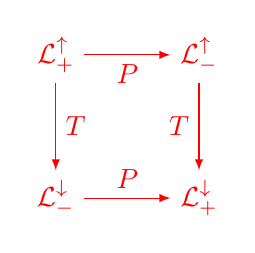
\begin{tikzpicture}[x=1mm,y=1mm, color=red]%
	\ifdefined\tikZlength\else\newlength{\tikZlength}\fi
	\setlength{\tikZlength}{0.15\linewidth}
	\coordinate (lo) at (-\tikZlength/2,\tikZlength/2);
	\coordinate (ru) at (\tikZlength/2,-\tikZlength/2);
	\coordinate (lu) at (lo |- ru);
	\coordinate (ro) at (lo -| ru);
	\node (nlo) at (lo) {$\mathcal{L}^\uparrow_+$};
	\node (nlu) at (lu) {$\mathcal{L}^\downarrow_-$};
	\node (nro) at (ro) {$\mathcal{L}^\uparrow_-$};
	\node (nru) at (ru) {$\mathcal{L}^\downarrow_+$};
	\draw[-latex] (nlo) -- node[below] {$P$} (nro);
	\draw[-latex] (nlo) -- node[right] {$T$} (nlu);
	\draw[-latex] (nlu) -- node[above] {$P$} (nru);
	\draw[-latex] (nro) -- node[left] {$T$} (nru);
\end{tikzpicture}%

\chapter{Aufzählungen mit \texttt{enumerate, itemize}\texorpdfstring{, \url{https://github.com/labenbmic1}}{}}
\label{chap:Aufzaehlungen}
\begin{enumerate}
\item Ich bin Nummer 1
\item Ich bin Nummer 2
\item Was bin ich?
\end{enumerate}
Oder mit \texttt{itemize}:
\begin{itemize}
\item First
\item[H] Was ist hier falsch :D
\item Third
	\begin{enumerate}
	\item Yeah 1
	\item Yeah 2
	\end{enumerate}
\end{itemize}
\lipsum[1-5] Test, des \verb|\marginpar[links]{rechts}|\marginpar[Notiz (l)]{Notiz (r)} Randes. (links, wenn links Rand ist, ansonst wird der Text rechts ausgegeben), 
\lipsum[1-1] mit \verb|\marginline{}|\marginline{Test, \cite{LabenbacherTeX}, \ref{subfig:Gleitumgebungen:mit subcaptionbox:A}} erfolgt immer eine Ausgabe (egal ob links rechts). Besser: \TUMstyle{package}{scrlayer-notecolumn}

\chapter{Richtiges Referenzieren mit \texttt{autoref, ref, subref, footref, eqref, pageref}}
\label{chap:Richtiges Referenzieren}
\begin{table}\centering
	\caption{Referenzierungsmöglichkeiten}
	\label{tab:Referenzieren:Referenzierungsmoeglichkeiten}
	\begin{tabular}{c|c|c|c}%
& \TUMstyle{1}{autoref} & 
\TUMstyle{1}{ref}  &
\TUMstyle{1}{special} \\
Part & 
\autoref{part:Gleitumgebungen in scrbook}	& 
\ref{part:Gleitumgebungen in scrbook} &\\
Chapter & \autoref{chap:Einfuehrung:Hauptklassen}	 &
\ref{chap:Einfuehrung:Hauptklassen} &\\
Section & \autoref{sec:Einfuehrung:Hauptklassen:Absatzauszeichnung} &
\ref{sec:Einfuehrung:Hauptklassen:Absatzauszeichnung} &\\
Table & \autoref{tab:Tabellen:A long table} & 
\ref{tab:Tabellen:A long table} &\\
Table & \autoref{subtab:Tabellen:mit latex-subtable:two} & 
\ref{subtab:Tabellen:mit latex-subtable:two} &
\subref{subtab:Tabellen:mit latex-subtable:two}\\
Figure & \autoref{fig:Gleitumgebungen:Grafik mit subcaptionbox ohne captionsetup (Standard: komafont)} & 
\ref{fig:Gleitumgebungen:Grafik mit subcaptionbox ohne captionsetup (Standard: komafont)} &\\
Figure & \autoref{subfig:Gleitumgebungen:mit subcaptionbox:D} & 
\ref{subfig:Gleitumgebungen:mit subcaptionbox:D} &
\subref{subfig:Gleitumgebungen:mit subcaptionbox:D}\\
Theorem & \autoref{theo:Theorem 1:theorem 1} & \ref{theo:Theorem 1:theorem 1}& \\
Lemma & \autoref{lem:Theorem 1:lemma 1} & \ref{lem:Theorem 1:lemma 1}& \\
Corollary & \autoref{cor:Theorem 1:corollary 1} & \ref{cor:Theorem 1:corollary 1}& \\
Definition &  \autoref{def:Theorem 1:definition 1} & \ref{def:Theorem 1:definition 1}& \\
Example &  \autoref{exam:Theorem 1:example 1} & \ref{exam:Theorem 1:example 1}& \\
Remark & \autoref{rem:Theorem 1:remark 1} & \ref{rem:Theorem 1:remark 1}& \\
Equation &  & \eqref{equ:Mathematik:sub-gesamt} & \eqref{subequ:Mathematik:sub-b} \\
Subsec.~\ref{subsec:Einfuehrung:Satzspiegelberechnung:Grundlagen:Weiterentwicklung} on page && \pageref{subsec:Einfuehrung:Satzspiegelberechnung:Grundlagen:Weiterentwicklung} &\\
Listing & \autoref{lst:introduction:3} & \ref{lst:introduction:3} & \\
	\end{tabular}
\end{table}
Nun gibt es noch \verb|\fullref|, \verb|\fulleqref| und \verb|\fullautoref| wo jeweils auch die Seite angegeben wird, z.\,B. letzer Befehl: \fullautoref{subtab:Tabellen:mit latex-subtable:two}. Vom Buch: \cite{LabenbacherTeX}, oder siehe Fußnoten: Mit ref: \ref{footnote:Tabellen:A footnote in the tableentry-firsthead}, Mit \verb|\footref| (KomaScript): \footref{footnote:Tabellen:A footnote in the tableentry-firsthead} (Bei Fußnoten kein autoref, da dies nicht unterstützt wird!). Der Style von \verb|\eqref| wird nicht beeinflusst im gegensatz zu \verb|\ref|, er ist immer \verb|\textup{...}| und \verb|\normalfont|. Würde man dies ändern wollen, d.h. so dass sich der Befehl wie \verb|\ref| verhält so müsste man in die Preamble folgendes ergänzen (Einfach von \TUMstyle{package}{amsmath} kopiert ohne \verb|\textup{...}| (zweite Zeile) und \verb|\normalfont| (dritte Zeile).):%
\begin{lstlisting}[style=LaTeX, caption={\LaTeX-Code für \ldots{}.}, label={lst:introduction:3}]
\makeatletter%
\renewcommand*\maketag@@@[1]{\hbox{\m@th #1}}%
\renewcommand{\eqref}[1]{{\tagform@{\ref{#1}}}}%
\makeatother%
\end{lstlisting}



\chapter{Mathematik mit/ohne \texttt{equbox}, und \texorpdfstring{\TUMstyle{package}{chemformula}}{chemformula}-Package}
\label{chap:Mathematik}
\begin{align}
\int\limits_{a}^{b} f \left( x \right) \dd{x} &= F(b) - F(a) \\
\pdv[n]{f}{x} &= \dfrac{x^{3}}{3} + \exp \left( -\lambda x \right) + \hypsine \left( x^{3} \right) + \exp \left( - \frac{\mathrm{i}}{x} \right) \notag\\
\sum\limits_{i=1}^{n} a_{n} &= e^{\mathrm{i} \pi } \cdot \sqrt[3]{n}  \xrightarrow{n \to \infty} \infty 
\end{align}
\begin{equbox}
	\begin{align}
	E=mc^2\label{equ:Mathematik:E = mc2}
	\end{align}%
\end{equbox}%
\begin{equbox}[Wenn es einen Titel bedarf. :D][breakable]
	\allowdisplaybreaks%
	\begin{align}%
	\int\nolimits_a^b \dd[3]{x} &= \int\limits_a^b \dd[3]{x}\\%
	\sum\nolimits_{n=1}^{\infty} &= \sum_{n=1}^\infty\\%
	\label{equ:Mathematik:Formel} \\%
	\ch{%
		RNO2 &<=>[ + e- ] RNO2^{-.} \\%
		RNO2^{-.} &<=>[ + e- ] RNO2^2-%
	} \\%
	a&=b
	\end{align}%
\end{equbox}%
Nun zum Paket siunitx: Man schreibt $a=\SI{5000}{\kilo\gram\metre\per\square\second}$ oder z.B. einfach mal etwas so wie $\si{\joule\per\mole\per\kelvin}$, $\si{\kilo\gram_{poly}\squared\per\mole_{cat}\per\hour}$ (für Hochzahlen muss cat als SI-Qualifier erklärt werden in der Preamble!), $\SI{3.00}{\MHz}$%
\begin{center}%
\ch{
	!($1s^22s^1$)( "\chlewis{180.}{Li}" ) +%
	!($1s^22s^22p^5$)( "\chlewis{0.90,180,270}{F}" ) %
	-> %
	!($1s^2$)( Li+ ) + !($1s^22s^22p^6$)( "\chlewis{0,90,180,270}{F}" {}- )%
}%
\end{center}%
Nun Subequations:%
\begin{subequations}%
	\label{equ:Mathematik:sub-gesamt}%
	\begin{align}%
	{\cal M}=&ig_Z^2(4E_1E_2)^{1/2}(l_i^2)^{-1}
	(g_{\sigma_2}^e)^2\chi_{-\sigma_2}(p_2)\nonumber\\
	&\times
	[\epsilon_i]_{\sigma_1}\chi_{\sigma_1}(p_1)
	\label{subequ:Mathematik:sub-a}
	\end{align}%
	\begin{gather}%
	\left\{
	abc123456abcdef\alpha\beta\gamma\delta 1234556\alpha\beta
	\frac{1\sum^{a}_{b}}{A^2}
	\right\}
	\label{subequ:Mathematik:sub-b}
	\end{gather}%
\end{subequations}%
Die Formel \eqref{equ:Mathematik:sub-gesamt} besteht aus \eqref{subequ:Mathematik:sub-a} und \eqref{subequ:Mathematik:sub-b}.\par%
Nun ein Beispiel einer Matrix mit \TUMstyle{package}{nicematrix}:%
\begingroup% Group: currently necessary for nicematrix (not in newest version anymore, but older ones)
\tikzexternaldisable%
\begin{gather}
	\hat{b} = \text{$%
		\begin{pNiceMatrix}[nullify-dots]
			0 			& 1		 	& 0			& \Cdots 	& 				&  		& \\
			\Vdots		& 0 		& \sqrt{2} 	& 0 		& \Cdots		&  		& \\
			& \Vdots	& 0			& \sqrt{3}	& 0				& \Cdots& \\
			& 		 	& \Vdots	& 0			& \Ddots		& 		& \\
			& 		 	& 		 	& \Vdots	&				& 		& \\
		\end{pNiceMatrix}
		$}
	,\qquad
	\hat{b}^\dagger = \text{$%
		\begin{pNiceMatrix}[nullify-dots]
			0 			& \Cdots 	&  			& 		 	& 				& \\
			1 			& 0 		& \Cdots 	&  			&				& \\
			0 			& \sqrt{2} 	& 0			& \Cdots 	&				& \\
			\Vdots		& 0 		& \sqrt{3}	& 0			& \Cdots		& \\
			& \Vdots 	& 0			& \Ddots	& 				& \\
			& 		 	& \Vdots 	& 			&				& \\
		\end{pNiceMatrix}
		$}.
\end{gather}%
\endgroup%
Now externalize a TikZ-picture again:\\%
{% Group: Reactivate externalization 
	\tikzset{external/export=true}%
	\tikzsetnextfilename{Figure-Einfuehrung-2}%
	\begin{tikzpicture}[x=1mm,y=1mm, color=TUMBlue]%
		\ifdefined\tikZlength\else\newlength{\tikZlength}\fi
		\setlength{\tikZlength}{0.15\linewidth}
		\coordinate (lo) at (-\tikZlength/2,\tikZlength/2);
		\coordinate (ru) at (\tikZlength/2,-\tikZlength/2);
		\coordinate (lu) at (lo |- ru);
		\coordinate (ro) at (lo -| ru);
		\node (nlo) at (lo) {$\mathcal{L}^\uparrow_+$};
		\node (nlu) at (lu) {$\mathcal{L}^\downarrow_-$};
		\node (nro) at (ro) {$\mathcal{L}^\uparrow_-$};
		\node (nru) at (ru) {$\mathcal{L}^\downarrow_+$};
		\draw[-latex] (nlo) -- node[below] {$P$} (nro);
		\draw[-latex] (nlo) -- node[right] {$T$} (nlu);
		\draw[-latex] (nlu) -- node[above] {$P$} (nru);
		\draw[-latex] (nro) -- node[left] {$T$} (nru);
	\end{tikzpicture}\\%
}%
And again with \TUMstyle{package}{nicematrix}:%
\begingroup% Group: currently necessary for nicematrix (not in newest version anymore, but older ones)
\tikzexternaldisable%
\begin{gather}
	\hat{b} = \text{$%
		\begin{pNiceMatrix}[nullify-dots]
			0 			& 1		 	& 0			& \Cdots 	& 				&  		& \\
			\Vdots		& 0 		& \sqrt{2} 	& 0 		& \Cdots		&  		& \\
			& \Vdots	& 0			& \sqrt{3}	& 0				& \Cdots& \\
			& 		 	& \Vdots	& 0			& \Ddots		& 		& \\
			& 		 	& 		 	& \Vdots	&				& 		& \\
		\end{pNiceMatrix}
		$}
	,\qquad
	\hat{b}^\dagger = \text{$%
		\begin{pNiceMatrix}[nullify-dots]
			0 			& \Cdots 	&  			& 		 	& 				& \\
			1 			& 0 		& \Cdots 	&  			&				& \\
			0 			& \sqrt{2} 	& 0			& \Cdots 	&				& \\
			\Vdots		& 0 		& \sqrt{3}	& 0			& \Cdots		& \\
			& \Vdots 	& 0			& \Ddots	& 				& \\
			& 		 	& \Vdots 	& 			&				& \\
		\end{pNiceMatrix}
		$}.
\end{gather}%
\endgroup%

\chapter{Theorem Teil 1 mit \texorpdfstring{\TUMstyle{package}{tcolorbox}}{tcolorbox}}%
\label{chap:Theorem 1}%
\lipsum[1-1]%
\begin{theorem}{Mittelwertsatz f\"{u}r $n$ Variable}{Theorem 1:Mittelwertsatz}%
	Es sei $n\in\mathbb{N}$, $D\subseteq\mathbb{R}^n$ eine offene Menge und $f\in C^{1}(D,\mathbb{R})$. Dann gibt es auf jeder Strecke $[x_0,x]\subset D$ einen Punkt $\xi\in[x_0,x]$, so dass gilt%
	\begin{equation*}%
	f(x)-f(x_0) = \operatorname{grad} f(\xi)^{\top}(x-x_0)%
	\end{equation*}%
\end{theorem}%
\begin{theorem*}{}{}%
	Ein Beispiel mit keiner Nummer.%
\end{theorem*}%
\begin{theorem}{}{}%
	Ein Beispiel mit keinem Titel.%
\end{theorem}%
\begin{lemma}{title :D}{Theorem 1:lemma 1}%
	Hallo Welt.
\end{lemma}%
\begin{corollary}{title :D}{Theorem 1:corollary 1}%
	Hallo Welt.
\end{corollary}%
\begin{proof}{}{Proof 1:proof 1}%
	\lipsum[1-3]
\end{proof}

\begin{definition}{title :D}{Theorem 1:definition 1}%
	\lipsum[1-1]
\end{definition}%
\begin{remark}{title :D}{Theorem 1:remark 1}%
	\lipsum[1-1]
\end{remark}%

\begin{theorem}{title :D}{Theorem 1:theorem 1}%
	\lipsum[1-1]
\end{theorem}%
\begin{proof*}{Titel?, zu Lemma \ref{lem:Theorem 1:lemma 1}}%
	\lipsum[1-1]
\end{proof*}
\begin{example}{}{Theorem 1:example 1}
Hello
\end{example}

\chapter{Theorem Teil 2 mit \texorpdfstring{\TUMstyle{package}{tcolorbox}}{tcolorbox}}%
\label{chap:Theorem 2}%
\begin{theorem}{title :D}{Theorem 2:theorem 2}%
	\lipsum[1-1]
\end{theorem}%
Dies ist das Theorem \nameref{theo:Theorem 1:Mittelwertsatz}, oder Theorem \ref{theo:Theorem 1:Mittelwertsatz}. \lipsum[1-1]%
\newpage%
\layout%
\newpage%


\newpage%
\KOMAoption{headheight}{27.2pt}% see .log file, after one miscalculation
\AfterCalculatingTypearea{%
	\TUMAfterCalculatingTypearea%
}\recalctypearea%
\chapter{Indices -- \texorpdfstring{\TUMstyle{package}{glossaries}}{glossaries}, todos -- \texorpdfstring{\TUMstyle{package}{todonotes}}{todonotes}, notes -- \texorpdfstring{\TUMstyle{package}{scrlayer-notecolumn}}{scrlayer-notecolumn}, Langer Header (sowas sollte man unterlassen aber so ginge es\ldots{}) :P.}%
\label{chap:IndicesTodosNotes}%
%\TUMstyle{number}{...} for emphasing text (or \TUMfont{number})
Der Mensch ist ein Tier, das Geschäfte macht; kein anderes Tier tut dies -- kein Hund tauscht Knochen mit einem anderen. \cite{LabenbacherTeX} Hello \gls{idx.people}, \gls*{idx.entry}, \Gls+{idx.entry.subentry}, \Gls{idx.entry.subentry.subsubentry}, \gls*[format=TUMindexnumber]{idx.animal}, 
\gls+{idx.beast}, 
\gls{fcp.aa}, \gls*{fcp.ab}, \gls+{fcp.ac}, \gls{fcp.ad}, \gls*{fcp.dd}, \gls+{fcp.da}, empty\glsadd[format=TUMindexnumber]{idx.empty}, %

L\\
La\todoMissing[caption={Missing.}]{I'm missing here\ldots.}\\
LaT\todoUnsure[caption={Unsure.}]{Unsure if that's good enough.}\\
LaTe\todoChange[caption={Change/Delete.}]{Please change this later on.}\\
LaTeX\todoInfo[caption={Info.}]{Nothing interesting.}\\
\LaTeX\todoImprovement[caption={Improvement.}]{Please Improve this code.}\\
\LaTeXe\\
\LaTeX3, \makenote[marginpar]{%.
	Bei \LaTeX3 steht ein wichtiger Text bzw. Bild in der Randnotiz:\\%
	\includegraphics[width=\linewidth]{help}\\%
	Wir \textit{können} mit \TUMstyle{package}{scrlayer-notecolumn} auch Umbrüche \textcolor{red}{ohne Probleme} behandeln.\par\medskip%
	Skip und weiter\ldots{}.%
}\makenote[marginpar]{An selben Stelle noch einmal führt dazu, dass der Text nach dem vorherigen ausgegeben wird ohne Überschneidung.}%
Es gibt zwei Arten sein Leben zu leben: Entweder so, als wäre nichts ein Wunder, oder so, als wäre Alles eines.\par\medskip%
Mit Hilfe von \verb|\makenote| kann Text in die Randspalte geschrieben werden. Im Gegensatz zu \verb|\todo| handelt es sich hier aber um einen \openautoquote{}wichtigen\closeautoquote{} Text und kann sowohl Seitenumbrüche händeln und die einzelnen Notizen überschneiden sich nicht. (Natürlich überschneiden sich todonotes mit den makenotes, aber die todos sind ja am Ende nicht mehr dabei.)

\begin{longtable}{C{0.25\textwidth}Z{p}{0.2\textwidth}{\raggedleft}l}%
	\caption{A long table}\label{tab:introduction:1}\\%
	\toprule%
	f-head & f-head & f-head \\%
	\midrule%
	\endfirsthead%
	\toprule%
	head & head & head \\%
	\midrule%
	\endhead%
	\midrule%
	foot & foot & foot \\%
	\bottomrule%
	\endfoot%
	\midrule%
	l-foot & l-foot & l-foot \\%
	\bottomrule%
	\endlastfoot%
	%% =========================== %%
	a&b\todoChange[caption={Change/Delete.}]{Please delete this part of the introduction.}&c\\%
	%% =========================== %%
\end{longtable}%
\begin{figure}%
	%\includegraphicshelp% *[options]
	%\includegraphicshelp[]% *[options]
	%\includegraphicshelp[angle=45]% *[options]
	\todoincludegraphics{Missing number one.}% *[options]
	\todoincludegraphics[]{Missing number two.}% *[options]
	\todoincludegraphics[angle=90]{Missing number three.}% *[options]
	\caption[Test 1]{Hier dann die Beschreibung des Bildes bitte rein. :P, und nochmals: Hier dann die Beschreibung des Bildes bitte rein.\todoChange[caption={Change/Delete.}]{Please delete this part of the introduction.} :P, Hier dann die Beschreibung des Bildes bitte rein. :P, Hier dann die Beschreibung des Bildes bitte rein. :P, Hier dann die Beschreibung des Bildes bitte rein. :P, Hier dann die Beschreibung des Bildes bitte rein. :P, Hier dann die Beschreibung des Bildes bitte rein. :P, Hier dann die Beschreibung des Bildes bitte rein. :P, \ldots{}.}%
	\label{fig:introduction:1}%
\end{figure}%
\newpage% only for index-test
\lstinputlisting[style=python, caption={Python-Code für \ldots{}.}, label={lst:introduction:1}]{listings/test.py}%

\section{Sub-(ind/todo)}%
\label{sec:introduction:Sub-indtodo}%
\ifdef{\idxadd}{}{\NewDocumentCommand{\idxadd}{O{}m}{\glsadd[#1]{idx.#2}}}%
\ifdef{\fcpadd}{}{\NewDocumentCommand{\fcpadd}{O{}m}{\glsadd[#1]{fcp.#2}}}%
\Gls{idx.people}, \gls[format=TUMindexnumberi]{idx.entry}, beast\idxadd{beast}, dog\idxadd{animal.dog}, \gls{fcp.ad}, \fcpadd[format=(TUMindexnumberi]{ba}
\newpage\glspl{idx.people}, \gls[format=TUMindexnumberi]{idx.animal}, \gls{idx.entry}, key\idxadd[format=TUMindexnumberi]{key}, electrician\glsadd{idx.people.electrician}, 
\newpage\gls{idx.entry}, \gls[format=(]{idx.people},\newpage{}A,\newpage{}\gls[format=)]{idx.people}, 
ba\fcpadd[format=)]{ba}, \gls[format=TUMindexnumber]{fcp.empty}, \gls{idx.LaTeX}, \gls{idx.LaTeX.file}, \gls{idx.LaTeX.class}, \gls{idx.LaTeX.package}, \gls{fcp.aa}, \gls{fcp.ab}, \gls{fcp.ac}, \gls{fcp.ad}, \gls{fcp.ba}, \gls{fcp.bb}, \gls{fcp.bc}, \gls{fcp.bd}, \gls{fcp.ca}, \gls{fcp.cb}, \gls{fcp.cc}, \gls{fcp.cd}, \gls{fcp.da}, \gls{fcp.db}, \gls{fcp.dc}, \gls{fcp.dd}, \gls{idx.dump}, \gls{idx.cinema}, \gls{idx.control}%

\lipsum[1-1] \gls{idx.entry.subentry} \gls*{idx.entry.subentry.subsubentry} \gls+[format=(]{idx.entry} %
\lipsum[1-3] Mensch\newline%
\lipsum[1-4] Mensch\todoImprovement[disable]{Everything that heightens the feeling of power in man, the will to power, power itself.}%
\lipsum[1-26] Mensch%\newline%
\lipsum[1-9] Mensch\gls[format=)]{idx.entry}\newline%
\lipsum[1-10] Mensch\gls[format=(]{idx.entry}\newline%
\lipsum[1-11] Mensch\gls[format=)]{idx.entry}\newline%
\lipsum[1-12] Mensch\gls[format=TUMindexnumberi]{idx.entry}\newline%
\lipsum[1-13] Mensch\gls[format=(TUMindexnumber]{idx.entry}%
\lipsum[1-8]\lipsum[1-18] \gls[format=)]{idx.entry}%
\lipsum[1-8]\gls{idx.entry}%

\begin{equation}
	a^2=b^2+c^2 \textrm{\todoChange{Delete this.}}
\end{equation}

\newpage\TUMStandardAreaMain%
\chapter[Nun wieder ein kurzer Titel.]{Nun wieder ein kurzer Titel, zumindest im Header, so sollte man es normalerweise machen.}\label{chap:Nun wieder ein kurzer Titel}%
Der Header sollte wieder klein sein. \glspl*{abb.shtml}, \gls+{abb.shtml}, \glspl{abb.shtml}\newpage
\gls{abb.a}\newpage\gls{abb.a}
\gls{abb.b}\newpage\gls{abb.a}
\gls{abb.b}\newpage\gls{abb.a}
\gls{abb.c}\newpage
\gls{abb.b}\newpage\gls{abb.a}
\gls{abb.b}\newpage\gls{abb.a}
\gls{abb.d}\newpage
\gls{abb.b}\newpage\gls{abb.a}
\gls{abb.b}\newpage\gls{abb.a}
\gls{abb.e}\newpage
\gls{abb.b}\newpage\gls{abb.a}
\gls{abb.b}\newpage\gls{abb.a}
\gls{abb.f}\newpage
\gls{abb.b}\newpage\gls{abb.a}
\gls{abb.b}\newpage\gls{abb.a}
\gls{abb.g}\newpage
\gls{abb.b}\newpage\gls{abb.a}
\gls{abb.b}\newpage\gls{abb.a}
\gls{abb.h}\newpage
\gls{abb.b}\newpage\gls{abb.a}
\gls{abb.b}\newpage\gls{abb.a}
\gls{abb.i}\newpage
\gls{abb.b}\newpage\gls{abb.a}
\gls{abb.b}\newpage\gls{abb.a}
\gls{abb.b}\newpage\gls{abb.a}
\gls{abb.j}\newpage
\gls{abb.b}\newpage\gls{abb.a}
\gls{abb.b}\newpage\gls{abb.a}
\gls{abb.k}\newpage
\gls{abb.b}\newpage\gls{abb.a}
\gls{abb.l}\newpage
\gls{abb.b}\newpage\gls{abb.a}
\gls{abb.b}\newpage\gls{abb.a}
\gls{abb.m}\newpage
\gls{abb.b}\newpage\gls{abb.a}
\gls{abb.b}\newpage\gls{abb.a}
\gls{abb.n}\newpage
\gls{abb.b}\newpage\gls{abb.a}
\gls{abb.b}\newpage\gls{abb.a}
\gls{abb.o}\newpage
\gls{abb.b}\newpage\gls{abb.a}
\gls{abb.b}\newpage\gls{abb.a}
\gls{abb.a}\newpage
\gls{abb.a}\newpage
\gls{abb.c}\newpage
\gls{abb.a}\newpage
\gls{abb.a}\newpage
\gls{abb.c}\newpage
\gls{abb.a}\newpage
\gls{abb.a}\newpage
\gls{abb.c}\newpage
\gls{abb.a}\newpage
\gls{abb.a}\newpage
\gls{abb.c}\newpage
\gls{abb.a}\newpage
\gls{abb.a}\newpage
\gls{abb.c}\newpage
\lipsum[1-30]%




%% end: LaTeX-Einfeuhrung.tex